\documentclass[12pt]{article}
\usepackage{report}
\usepackage[acronym]{glossaries}
\usepackage{rotating}
\usepackage{float}
\usepackage{siunitx}
\usepackage{array}
\usepackage[justification=centering]{caption}
\usepackage{booktabs}
\usepackage[table,xcdraw]{xcolor}
\usepackage{chngcntr}
\usepackage[utf8]{inputenc}
\usepackage{geometry}
\usepackage{array}
\usepackage{longtable}
\usepackage{lscape} % For landscape orientation if needed
\geometry{a4paper, margin=1in}
\renewcommand{\arraystretch}{1.2} % Adjust row height
\usepackage{xcolor} % Allows custom colors
\usepackage[colorlinks=true, linkcolor=blue, urlcolor=red, citecolor=green]{hyperref}

\title{Project proposal format For B.Sc. CSIT/BIT, TU, IOST}
\author{Prakash Neupane}
\date{\today}

\begin{document}
\pagenumbering{roman} % Roman page numbers

% Title page (Design in your own way)

\addcontentsline{toc}{section}{TITLE PAGE}
\thispagestyle{empty} % This will hide page number in title page


% Title page (Design in your own way)

{
	\thispagestyle{empty}
	\centering
	\normalsize
	  
        
\includegraphics[width=1.3in]{Images/PUClogo.png}\\

	{PREMIER UNIVERSITY}\\
	{DEPARTMENT OF COMPUTER SCIENCE AND ENGINEERING}\\
	
	\\[1.5cm]
	{\textit{A Project Report On}\\
	{\bf YOUR project Title Goes Here in UPPER CASE}\\[1.5cm]

     {\bf Course Title:} Software Development\\
     {\bf Course Code:}  CSE 364\\[1.5cm]

        Submitted To:\\
	   Faculty Name \\
          Designation \\
          Department of Computer Science and Engineering\\[1.5cm]
    
	% ~
	
	Submitted By:\\
	{\bf Full Name} (PU Exam Roll No)\\
        {\bf Full Name} (PU Exam Roll No)\\
	{\bf Full name} (PU Exam Roll No)\\[3.5cm]
	% ~
	
	September, 2024
	
}

}

%%% Local Variables:
%%% mode: plain-tex
%%% TeX-master: t
%%% End: % Ensure this file exists and is correctly formatted


% Table of contents
\newpage
{
  \setlength{\parskip}{0em}
  \renewcommand\contentsname{TABLE OF CONTENTs} % This will change heading text
  \tableofcontents \addcontentsline{toc}{section}{TABLE OF CONTENTS}
}

% List of figures - if any
\newpage
\listoffigures 
\addcontentsline{toc}{section}{LIST OF FIGURES}

% List of tables - if any
\newpage
\listoftables 
\addcontentsline{toc}{section}{LIST OF TABLES}
\pagenumbering{arabic}

\newpage
\section{Introduction}
Read some papers to begin and develop your writing style.
This section provides an overview of the project, including its significance and the motivation behind choosing the topic. Explain the broader context and relevance of the project, highlighting its potential impact on a specific field or problem area. Briefly describe what the project aims to achieve and the scope of work involved

Online vehicle rental systems are popular these days~\cite{vehicle}.
In the introduction, provide background information on the topic of your project. Explain the context and relevance of the problem you are addressing. Briefly state the purpose and scope of your project proposal. The introduction should capture the reader's interest and provide a high-level overview of what the proposal will cover~\cite{ref1}
 % Ensure this file exists and is correctly formatted
\section{Objectives} 
What problem does this project aim to solve?

Specify the goals and intended outcomes.

\section{Background and Motivation}
Why is this problem important or relevant?

\subsubsection{Literature Review}
    
Briefly outline any prior work, challenges, or opportunities in this area.
\section{Problem Statement}
Clearly define the problem or question the project seeks to address.
    
Specify how the solution will be evaluated (e.g., accuracy, speed, precision).


Sample of figure for problem statement:

\url{https://www.pi.exchange/hs-fs/hubfs/KH%20Article%20Assets/image-20230707-054308.png?width=500&height=333&name=image-20230707-054308.png} 
\section{Data Description}
 Source of data (public datasets, proprietary, synthetic, etc.).
 
Type of data (structured, unstructured, time series, etc.).

Data preprocessing or cleaning requirements.
\section{Methodology}
 Proposed machine learning approach (e.g., supervised learning, unsupervised learning, deep learning).
    
Algorithms/models under consideration.

Tools, libraries, and frameworks you plan to use.

\begin{figure}[h]
    \centering
    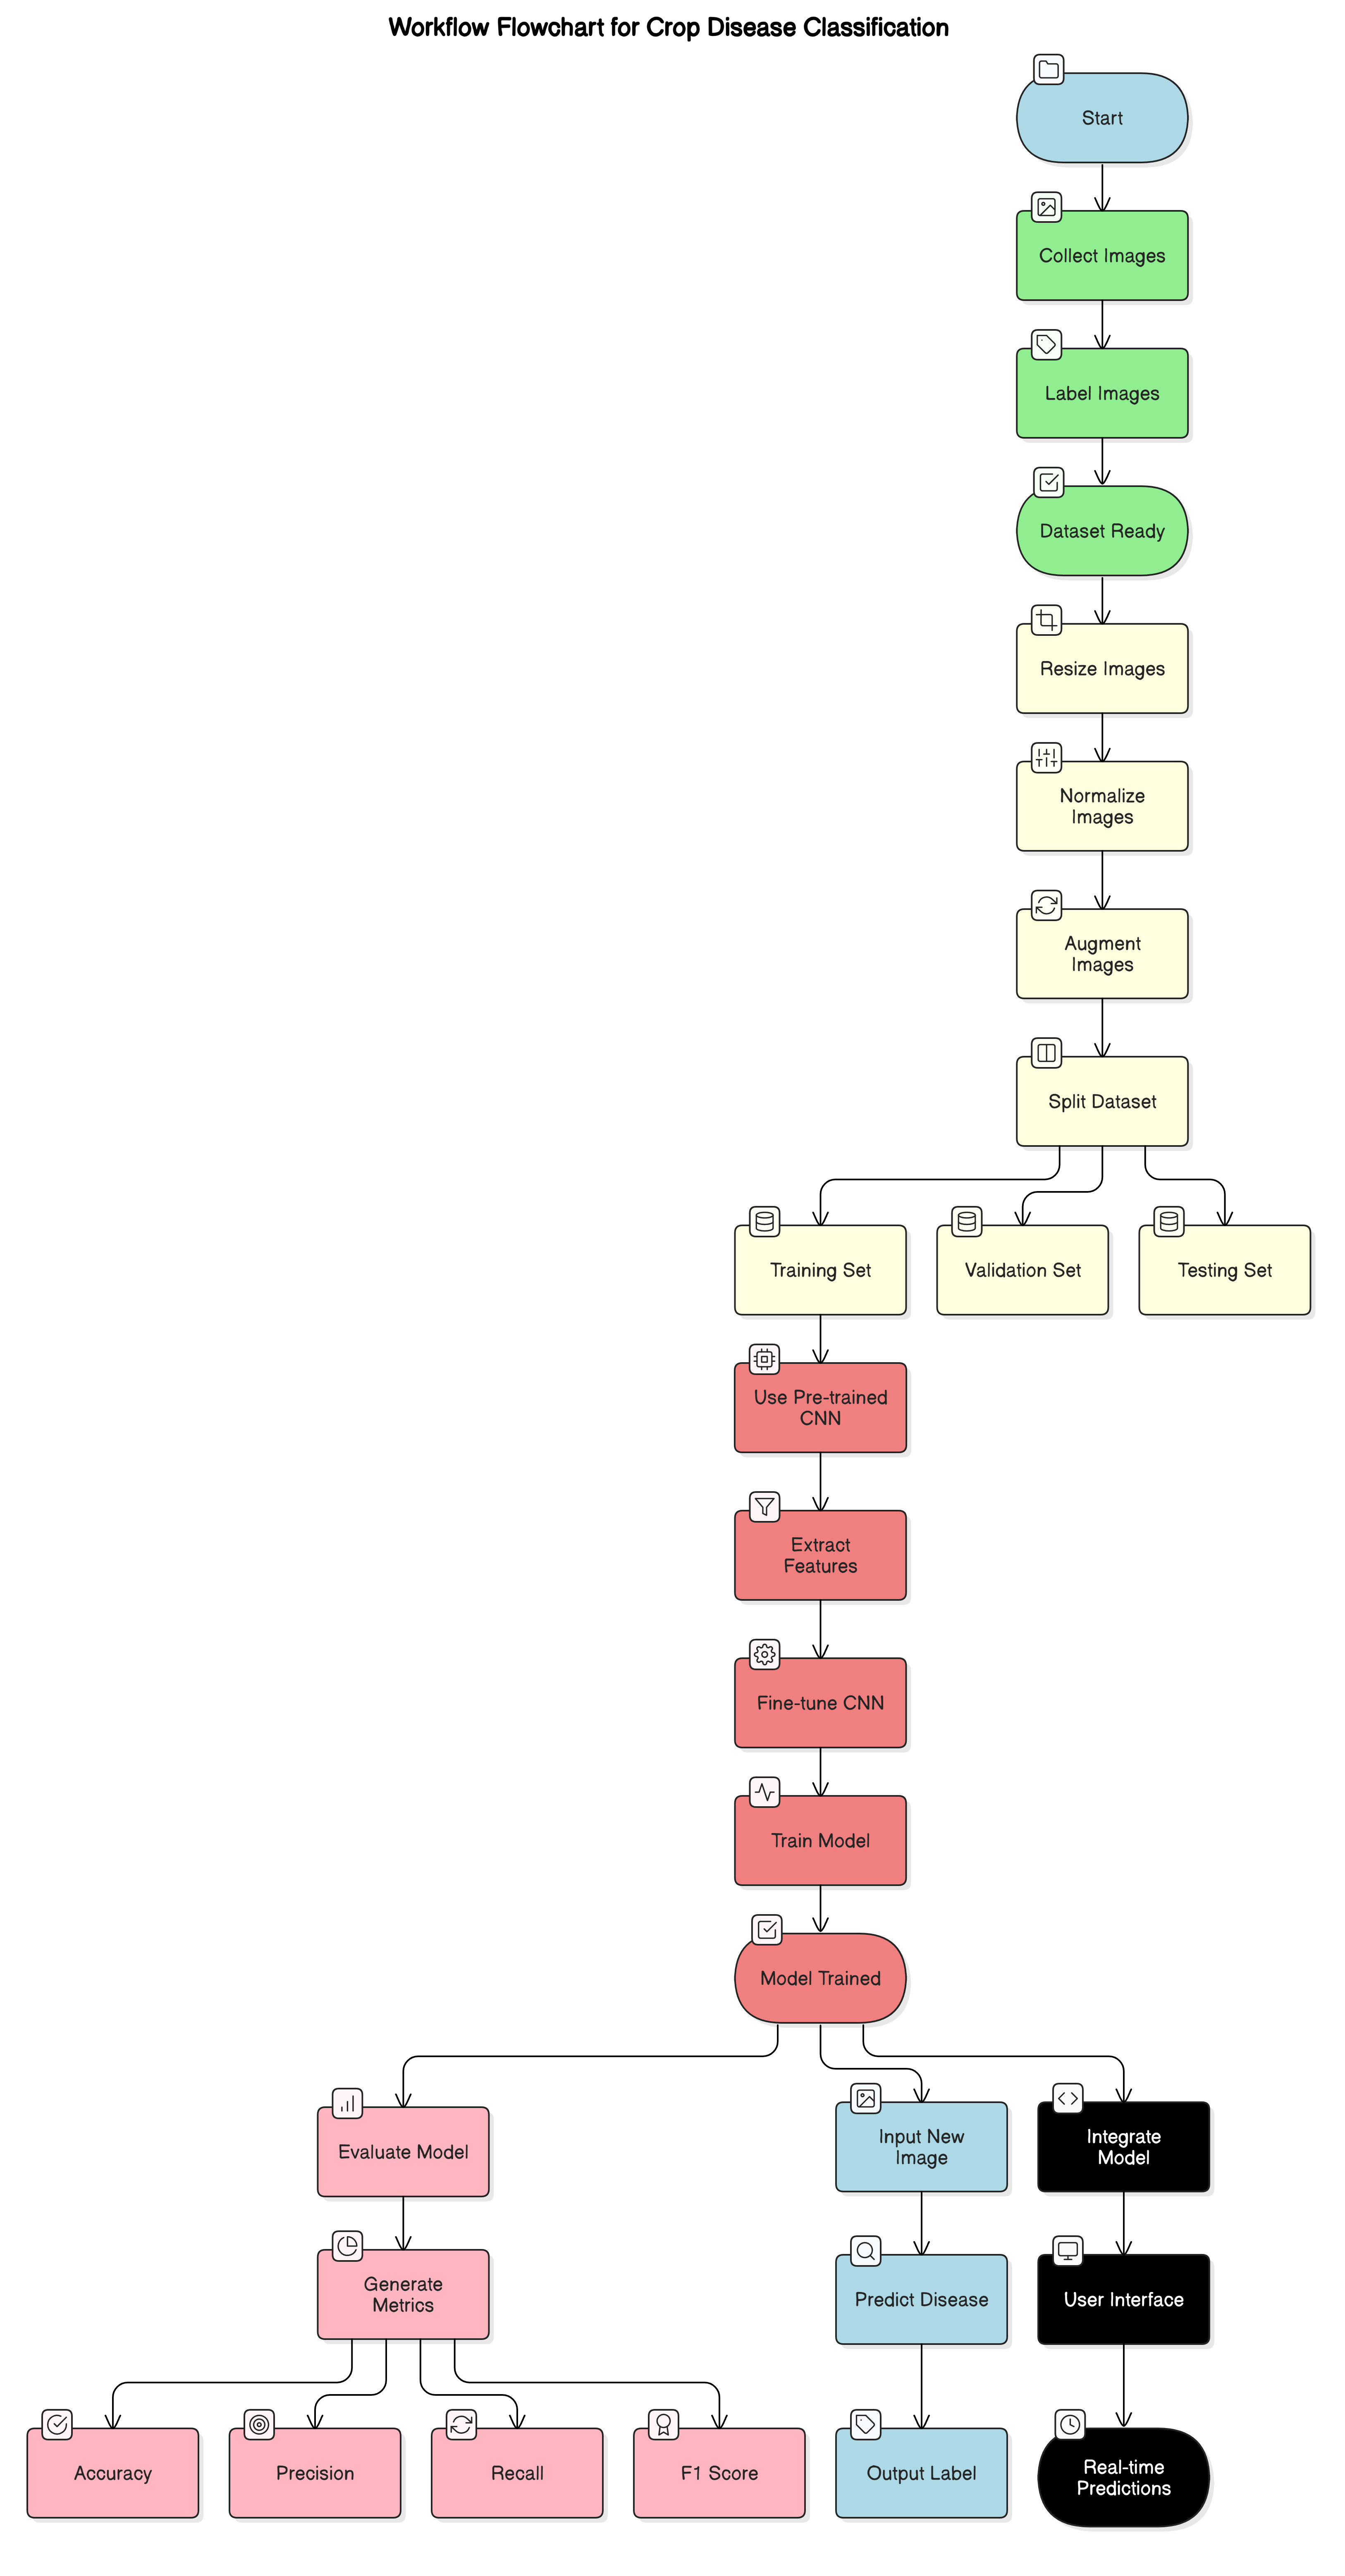
\includegraphics[width=0.5\linewidth]{Images/flow.png}
    \caption{Caption}
    \label{fig:enter-label}
\end{figure}

\begin{table}[h]
    \centering
    \caption{sample Cost-Benefit Analysis of the Proposed Project}
    \begin{tabular}{@{}llcc@{}}
        \toprule
        \textbf{Item} & \textbf{Description} & \textbf{Cost (\$)} & \textbf{Benefit (\$)} \\ \midrule
        Development Costs & Software Development & 15,000 & - \\
        Hardware Costs & Servers and Equipment & 5,000 & - \\
        Training Costs & User Training Sessions & 2,000 & - \\
        Maintenance Costs & Annual Maintenance & 1,000 & - \\
        \midrule
        \textbf{Total Costs} &  & \textbf{23,000} & - \\ \midrule
        Increased Efficiency & Time Savings & - & 30,000 \\
        Improved User Satisfaction & User Feedback & - & 10,000 \\
        Revenue Increase & New Customers & - & 20,000 \\
        \midrule
        \textbf{Total Benefits} &  & - & \textbf{60,000} \\ \midrule
        \textbf{Net Benefit} &  & \textbf{23,000} & \textbf{37,000} \\ 
        \bottomrule
    \end{tabular}
    \label{tab:cost-benefit}
\end{table}

 


\url{https://www.onlinegantt.com/#/gantt} to create a Gantt chart as per our need.
  

\section{Evaluation Metrices}
How will you measure success?

Common metrics: accuracy, precision, recall, F1 score, RMSE, etc.
\section{Implementation Plan}

Steps or phases of the project (data collection, preprocessing, model training, testing, deployment).
    
Estimated timeline for each phase.
\section{Expected Outcome}
What are the tangible deliverables of the project (e.g., predictive model, visualization, insights)?
    
Include potential business or research implications.
\input{sec/Societal_and_Cultural_Impact}
\section{Milestone}
\begin{figure}[H]
    \centering
    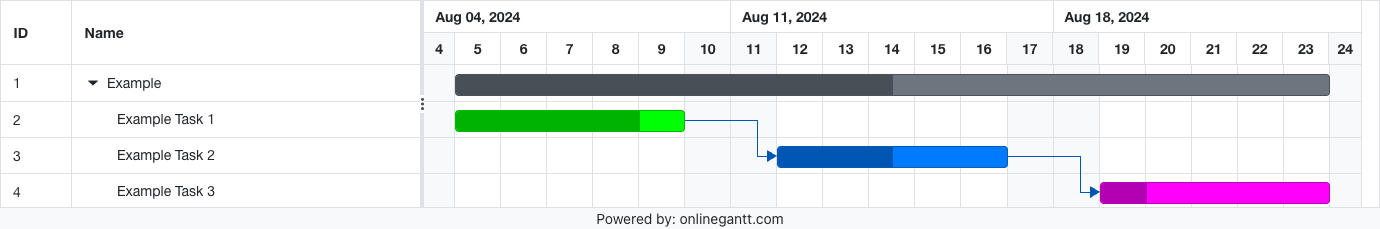
\includegraphics[width=1\linewidth]{Images/gantt.png}
    \caption{Sample Gantt Chart demonstrating schedule feasibility}
    \label{fig:enter-label}
\end{figure}
% References
\newpage
\phantomsection
\addcontentsline{toc}{section}{REFERENCES}
\nocite{ref1, ref2, ref3, ref4, ref5}
\bibliographystyle{IEEEtran}   % Keep this as IEEE style (if applicable)
\bibliography{biblio}          % Ensure 'biblio.bib' exists and contains all the references
\end{document}
